%%%%%%%%%%%%%%%%%%%%%%%%%%%%%%%%%%%%%
% Stylish Article
% LaTeX Template
% Version 2.0 (13/4/14)
%
% This template has been downloaded from:
% http://www.LaTeXTemplates.com
%
% Original author:
% Mathias Legrand (legrand.mathias@gmail.com)
%
% License:
% CC BY-NC-SA 3.0 (http://creativecommons.org/licenses/by-nc-sa/3.0/)
%
%%%%%%%%%%%%%%%%%%%%%%%%%%%%%%%%%%%%%%%%%

%----------------------------------------------------------------------------------------
%	PACKAGES AND OTHER DOCUMENT CONFIGURATIONS
%----------------------------------------------------------------------------------------

\documentclass[fleqn,10pt]{SelfArx} % Document font size and equations flushed left
\usepackage[spanish]{babel}

%----------------------------------------------------------------------------------------
%	COLUMNS
%----------------------------------------------------------------------------------------

\setlength{\columnsep}{0.55cm} % Distance between the two columns of text
\setlength{\fboxrule}{0.75pt} % Width of the border around the abstract

%----------------------------------------------------------------------------------------
%	COLORS
%----------------------------------------------------------------------------------------

\definecolor{color1}{RGB}{0,0,90} % Color of the article title and sections
\definecolor{color2}{RGB}{0,20,20} % Color of the boxes behind the abstract and headings

%----------------------------------------------------------------------------------------
%	HYPERLINKS
%----------------------------------------------------------------------------------------

\usepackage{hyperref} % Required for hyperlinks
\usepackage{cite}
\hypersetup{hidelinks,colorlinks,breaklinks=true,urlcolor=color2,citecolor=color1,linkcolor=color1,bookmarksopen=false,pdftitle={Title},pdfauthor={Author}}

%----------------------------------------------------------------------------------------
%	ARTICLE INFORMATION
%----------------------------------------------------------------------------------------

\JournalInfo{Taller de Biotecnología Animal, 2014-I} % Journal information
\Archive{Review} % Additional notes (e.g. copyright, DOI, review/research article)

\PaperTitle{Transfección en Animales} % Article title

\Authors{Juan Manuel Iglesias Artola\textsuperscript{1}, Gianfranco Villamonte Cuneo\textsuperscript{1}} % Authors
\affiliation{\textsuperscript{1}\textit{Facultad de Ciencias Biológicas, Universidad Ricardo Palma, Lima, Peru}} % Author affiliation
%\affiliation{\textsuperscript{2}\textit{Department of Chemistry, University of Examples, London, United Kingdom}} % Author affiliation
\affiliation{*\textbf{Correspondencia}: jmanuel9112@icloud.com / giancuneo@gmail.com } % Corresponding author


%----------------------------------------------------------------------------------------
%	ABSTRACT
%----------------------------------------------------------------------------------------

\Abstract{La transfección es el proceso de introducir nucleótidos en una célula, cuyo producto es la transgénesis. Existen múltiples métodos biológicos , físicos y químicos que permiten realizar esta introducción de nucleótidos. Además de la aparicion de múltiples métodos nuevos de transfección en los últimos años, su eficiencia se sigue incrementando. Esto ha permitido la aparición sin precedentes de un sinnúmero de aplicaciones (biomédicas, alimenticias, etc.) que plantean nuevos debates éticos y generan la necesidad de modernizar la reglamentación relacionada.  }


\Keywords{transfección --- transgénicos --- bioética} % Keywords - if you don't want any simply remove all the text between the curly brackets
\newcommand{\keywordname}{Palabras clave} % Defines the keywords heading name

%----------------------------------------------------------------------------------------

\begin{document}

\flushbottom % Makes all text pages the same height

\maketitle % Print the title and abstract box

\tableofcontents % Print the contents section

\thispagestyle{empty} % Removes page numbering from the first page

%----------------------------------------------------------------------------------------
%	ARTICLE CONTENTS
%----------------------------------------------------------------------------------------

\section{Introducción} 

Con la transfección se ha logrado la capacidad de expresar genes de interés en células eucariotas. Esta capacidad ha permitido obtener un mejor entendimiento de la biología celular, la biología molecular y la genética de las células. Al expresar proteínas en células de mamíferos, se ha podido entender aspectos detallados de la síntesis protéica, las interacciones entre proteínas, los efectos de las mutaciones en su función, y las interacciones intercelulares. Además, esta tecnología ha llevado al desarrollo de animales trangénicos, a la fertilización \textit{in vitro}, y a la posibilidad de usar la tranferencia de genes para tratar desórdenes genéticos.

Los virus fueron por mucho tiempo la forma más conveniente de transferir genes a células mamíferas. En 1973 Graham y van der Eb \cite{Graham:1973aa} utilizaron el adenovirus 2 para transfomar células de rata, mientras que en 1984 Cepko et al. \cite{Cepko:1984aa} desarrollaron un retrovirus murínico para la introducción de secuencias de DNA en células mamíferas. Si bien los virus constituyen un medio eficiente para lograr la transfección \textit{in vitro}, la construcción de los vectores es laboriosa, consume tiempo, y tiene diversas limitaciones para su uso \textit{in vivo}.

Si bien la transfección por medio de vectores virales es altamente eficiente, se han desarrollado también otros métodos. Los trabajos realizados por Pagano et al. fueron pioneros en su área al lograr una alta transferencia de genes a células mamíferas utilizando dietilaminoetil-dextrano (DEAE-D) mezclado con RNA y DNA  \cite{McCutchan:1968aa, Pagano:1967aa}. Después, se demostró que otros métodos también son eficaces: la encapsulación de DNA utilizando liposomas \cite{Fraley:1980aa, Wong:1980aa, Straubinger:1983aa, Fraley:1981aa}, la fusión inducida por polietilenglicol del DNA en los eritrocitos fantasma \cite{Straus:1980aa}, la electroporación \cite{Neumann:1982aa}, los coprecipitados de fosfato de calcio/DNA \cite{Wigler:1979aa}, y los policationes/dimetil sulfóxidos \cite{Kawai:1984aa}. Sin embargo, la eficiencia de los métodos utilizados varía con respecto a las tipos celulares y en general, no fueron muy eficientes y presentaban una alta toxicidad celular.

En la actualidad existen tres grandes grupos de métodos que pueden ser utilizados \cite{Kim:2010aa}: \textit{a)} los métodos biológicos, \textit{b)} los métodos químicos y \textit{c)} los métodos físicos. En cada uno de estos grupos existen métodos que se pueden emplear para producir una transfección pasajera o una integración estable en el genoma del hospedero. En este minireview se resumen las estrategias experimentales más generales, sus aplicaciones y las implicaciones bioéticas que puede tener la transfección de células animales.

\section{Métodos de Transfección}
Se han desarrollado diversas técnicas de transfección que cumplen con el propósito de transferir ácidos nucléicos al interior de las células. Existen ciertas características que permiten una transfección exitosa, estas son: alta eficiencia en el transporte del ácido nucléico a la ubicación celular apropiada (el núcleo para el DNA plasmídico y el citoplasma para el RNA); baja toxicidad celular; mínima interferencia con la fisiología celular normal; uso sencillo y que sea reproducible \cite{Schenborn}. Para el caso de la transfección génica utilizada para terapias se deben tomar consideraciones adicionales tales como la vida-media y el transporte a un tipo celular específico. En esta sección se discuten los tres principales métodos de transfección, los métodos biológicos, químicos y físicos

\subsection{Métodos biológicos}
El método más utilizado en la investigación clinical es el de la transfección mediada por virus, también conocida como transducción \cite{Pfeifer:2001aa}. Este método es altamente eficiente y permite la expresión sostenible del transgen \textit{in vivo} debido a la naturaleza viral de la integración en el genoma del huésped. Por ejemplo, se ha utilizado el virus de la leucemia murina (MLV)  como vector viral para establecer la expresión sostenible de genes de interés en humanos \cite{Hacein-Bey-Abina:2002aa, Roesler:2002aa}. El MLV integra su DNA en el genoma del hospedero, el cual es posteriormente expresado. El DNA del MLV integrado se replica con el genoma del hospedero, lo que permite la expresión sostenible del gen de interés.

La citotoxicidad y la inmunogenicidad representan las mayores desventajas de la transfección mediada por virus. La introducción del vector viral puede causar una reacción inflamatoria y una mutación insercional, debido a que los vectores virales se integran de manera azarosa al genoma del hospedero, lo cual puede afectar a genes supresores de tumores, activar oncogenes, o interrumpir genes esenciales \cite{Woods:2003aa}. Otra desventaja de este método es que la cápside de un virus tiene espacio limitado para que un gen extraño continúe siendo infectivo. 

\subsection{Métodos químicos}
Los métodos de transfección químicos son los más utilizados en el área de investigación y fueron los primeros en ser utilizados para introducir genes foráneos a células mamíferas \cite{Schenborn2000}. Los métodos químicos utilizan en su mayoría polímeros catiónicos, fosfato de calcio, lípidos catiónicos (el primer método utilizado) o amino ácidos catiónicos \cite{Schenborn2000, Holmen:1995aa, Washbourne:2002aa}. En líneas general el principio detrás de la transfección por métodos químicos es el mismo. Los compuestos utilizados están cargados positivamente lo que les permite formar complejos con los grupos fosfatos, cargados negativamente, de los ácidos nucléicos. Se piensa que esto permite la aposición de los complejos con la membrana celular que tiene carga negativa. Se desconoce el mecanismo exacto de como estos complejos pasan por la membrana celular; sin embargo, se considera que la internalización se produce por endocitosis y fagocitosis. Una vez que el DNA ingresa a la célula, este debe ser llevado al núcleo para ser expresado y, una vez más, no se conoce el mecanismo de traslocación al núcleo \cite{Kim:2010aa}.



\section{Aplicaciones de la Transfección}

La transfección es una herramienta para la modificación genética. Gracias a sus múltiples métodos es posible realizar innumerables aplicaciones como:
\begin{itemize}[noitemsep] % [noitemsep] removes whitespace between the items for a compact look
\item \textbf{Estudios Genéticos}: Genes 'knockout' o 'knockdown' para estudiar su expresión fenotípica.
\item \textbf{Terapia Génica}: Cura de enfermedades.
\item \textbf{Proteínas Recombinantes}: Uso de animales como 'bio-fábricas'.
\item \textbf{Alimentos Transgénicos}: Modificaciones genéticas principalmente para alimentación.
\item \textbf{Mascotas transgénicas}: Peces brillantes, gatos hipoalergénicos, etc.
\end{itemize}

\subsection{Estudios Genéticos}

La transfección puede ser útil para el estudio del funcionamiento de genes. Esto se puede realizar por varios medios: introduciendo un gen de otro organismo (transgenésis), mediante un knockout o knockdown que anule la expresión de un gen \cite{cryanin2004}, aumentando la expresión del gen de estudio \cite{yanni2004laboratory}, o alterando la estructura de la proteína que codifica \cite{ripps1995transgenic}.

De esta manera, este procedimiento ha permitido la realización de estudios sobre el funcionamiento de diversos genes humanos, principalmente con fines médicos.

Estas investigaciones incluyen el análisis de la influencia genética en trastornos psicológicos y neurodegenerativos, mediante la evaluación del fenotipo producido utilizando mecanismos de transfección (principalmente utilizando modelos murinos). Así vemos que la transfección ha permitido evaluar el impacto de la reducción de la enzima SOD-1 en la neurodegeneración producida en la Esclerosis Lateral Amiotrófica (ELA) \cite{ripps1995transgenic}. Asimismo, ha permitido el estudio de la relación de diversos receptores de neurotransmisores con la depresión \cite{cryanin2004}, el autismo, la esquizofrenia, el Alzheimer, la enfermedad de Huntington, entre otros \cite{anthe2002}.

La transfección también ha permitido evaluar el impacto de los genes en la regulación enzimática del metabolismo de lipidos, relacionada con enfermedades cardio-vasculares como la aterosclerosis\cite{yanni2004laboratory}


\subsection{Terapia Génica}

La terapia génica es una importante aplicación de la transfección a la medicina. Muchos de sus usos continuan en experimentación \textit{'in vitro'} o en animales, sin embargo, este campo tiene un gran potencial:
\begin{itemize}[noitemsep] % [noitemsep] removes whitespace between the items for a compact look
\item \ Cáncer
\item \ Enfermedades congénitas
\item \ Curación de heridas , quemaduras y otras afecciones epiteliales
\end{itemize}

La terapia génica se puede emplear para curar diversos tipos de cáncer mediante múltiples métodos. Uno de estos métodos es el de 'vacunación' anti-tumoral. Este consiste en utilizar la transfección para producir antígenos asociados al crecimiento tumoral. Además, se puede utilizar esta tecnología para inducir la producción de citoquinas que inhiban la angiogénesis. Asimismo, se puede usar para inducir el metabolismo de protoxinas por las células tumorales, haciendo que los medicamentos contra el cáncer sean de un impacto más directo y controlado\cite{Vile, Seung}.

La terapia génica puede asimismo ser utilizada para suprimir o controlar enfermedades congénitas, o aliviar sus síntomas, evitando a su vez los efectos secundarios que podría producir el uso de fármacos \cite{Spink}

En el caso de quemaduras, cortes, o afecciones epiteliales provocadas por diversas enfermedades (como el acné o el lupus eritematoso), muchas veces, la curación es lenta y deja muchas cicatrices debido a la ausencia o a la baja producción de factores de crecimiento. La transfección en tejidos epiteliales, probada a la fecha sólo en cultivos celulares y ratones, ha comprobado ser útil tanto para fomentar la regeneración de dichos tejidos, como para inducir su vascularización y reducir las cicatrices \cite{branskigene2006, Reinhart, strulovicihuman2007}.

\subsection{Proteínas Recombinantes}

Uno de los principales objetivos de la modificación genética de animales es la producción masiva de proteínas. Al buscarse en estos casos la producción, en lugar de la expresión en el animal en sí, la modificación genética en estos casos se enfoca en la leche de diversos mamíferos(ovejas, cabras, vacas, chanchos, entre otros).  Esta producción masiva se concentra en proteínas humanas de aplicación biomédica como algunos factores de coagulación, fibrinógeno, colágeno, enzimas y anticuerpos de origen humano; además de en la producción de proteínas de origen viral que podrían servir para inmunizar a las personas ante diversas enfermedades(ver cuadro\ref{cuadro1})\cite{Durocher15012002, Koszarycz2004, niemann2007transgenic, houdebine2009production}. 


\begin{table*}[t!]
\centering
\begin{tabular}{|l|c|c|} \hline
\textbf{Proteína} & \textbf{Enfermedad/Objetivo} & \textbf{Animal} \\ \hline
Activador Tisular del Plasminógeno (t-PA) &Trombosis & Cabra, ratón \\ \hline
Anti-CD137 & Enfermedades autoinmunes & Cabra \\ \hline
Albúmina de suero humano (HSA) & Mantenimiento de volumen sanguíneo & Ratón, vaca \\ \hline
$\alpha$-lacta albúmina & Anti-infección & Vaca \\ \hline
$\alpha$-1 antitripsina ($\alpha$-AT) & Deficiencia lleva a enfisema & Oveja \\ \hline
$\alpha$-glucosidasa & Enfermedad de Pompe & Conejo \\ \hline
Antitrombina 3 (ATIII) & Trombosis & Cabra \\ \hline
CFTR & Fibrosis Quística & Oveja , ratón \\ \hline
Calcitonina humana & Osteoporosis & Conejo \\ \hline
Colágeno I & Reparación de Tejidos & Vaca \\ \hline
Colágeno II & Artritis reumatoidea & Vaca \\ \hline
Decarboxilasa del ác. glutámico & Diabetes Tipo I & Cabra, ratón \\ \hline
Factor VIII & Hemofilia & Cerdo, oveja \\ \hline
Factor IX & Hemofilia & Cerdo, oveja, vaca \\ \hline
Fibrinógeno & Curación de heridas & Oveja, vaca \\ \hline
Lactoferrina & Infección artrítica o infección del tracto gastrointestinal & Vaca \\ \hline
msp-1 & Malaria & Ratón \\ \hline
Pro542 & VIH & Cabra, ratón \\ \hline
\end{tabular}

\caption{Proteínas producidas en diversos animales transgénicos \cite{Koszarycz2004, niemann2007transgenic, houdebine2009production}}
\label{cuadro1}
\end{table*}


\subsection{Alimentos Transgénicos}

La nutrición es una necesidad fisiológica básica para el ser humano\cite{maslow1943theory}. Por ello, el desarrollo de mejoras en las propiedades nutricionales de los alimentos es una prioridad para la humanidad. Tradicionalmente estas mejoras se han conseguido mediante la selección artificial, es decir, eligiendo a animales con características deseadas para incrementarlas o mantenerlas mediante su cruce. Sin embargo, esta técnica demora mucho tiempo y no siempre se obtienen todas las características deseadas. En la actualidad es posible realizar estas mejoras mucho más rápido y con total precisión, gracias a la tranfección.

Un importante rubro alimenticio en el que se enfoca la transfección es el de la leche. La leche es un alimento muy consumido a nivel mundial. No obstante, mucha gente tiene problemas con su consumo, debido a la intolerancia a la lactosa, la cual se encuentra en 5\% (aprox.) en la leche. Además, pese a tener una alta concentración de proteínas, no todas son de alta calidad por lo cual, no todas nutren de la misma forma a quien la consume. Por otro lado, la leche tiene una alta proporción de grasa (3-5\% (aprox.)). No obstante, todas esas deventajas se pueden superar mediante la transfección\cite{yom1993genetic}. 

Así,por ejemplo, la inhibición de la expresión de la acetil co-A carboxilasa, que se encarga de sintetizar grasa en las glándulas ,mamarias, puede reducir la concentración de grasa de la leche. Otra modificación importante, sería la de inhibir la producción de $\alpha$-lactalbúmina, la cual está relacionada con la síntesis de la lactosa, con lo cual se puede obtener leche con una concentración muy reducida o libre de ella. Además, la inhibición de la $\beta$-lactoglobulina en la leche de rumiantes puede eliminar las alergias relacionadas a su consumo, y otros ejemplos como el de la expresión de lisozima humana en la leche (proteína con cualidades anti-patogénicas y mejoradora de la flora intestinal) puede mejorar en gran medida la calidad nutricional de la leche\cite{yom1993genetic, pintado1998transgenesis, maga2006consumption}.

También se ha utilizado la transfección para mejorar la cantidad de carne en animales. Esta tecnología se ha aplicado principalmente en peces, puesto que los métodos de transfección han sido más eficientes en ellos hasta la fecha. Quizá el caso más conocido sea el del salmón. Este animal ha sido modificado para expresar una mayor concentración de la hormona del crecimiento. Esto permite un crecimiento mucho mayor en poco tiempo (ver fig\ref{salmon})\cite{berkowitz1994transgenic, ledford2013transgenic}.

\begin{figure}[ht]\centering
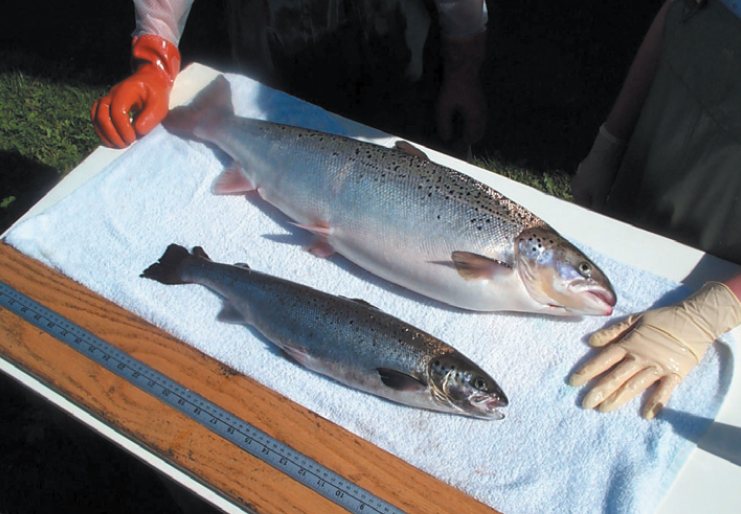
\includegraphics[width=\linewidth]{images/salmon}
\caption{Comparación del crecimiento de un salmón silvestre y un salmón transgénico con incremento en la expresión de la GH(Hormona del Crecimiento)\cite{berkowitz1994transgenic, ledford2013transgenic}}
\label{salmon}
\end{figure}

\subsection{Mascotas Transgénicas}
    
    La transfección permite la obtención de mascotas con características deseables comercialmente que, sin embargo, no se encuentren en estado natural. Estos han creado un nuevo nicho de mercado con un enorme potencial de crecimiento. 
    
    Un ejemplo muy interesante de mascotas transgénicas es el de los peces transgénicos. Inicialmente, Gong y colaboradores en la Universidad de Singapur, modificaron "peces cebra" (\textit{Danio rerio}) para expresar las proteínas fluorescentes GFP (proteína verde fluorescente), YFP (proteína amarillo fluorescente) y RFP (proteína rojo fluorescente) que actúan en asociación con el gen \textit{mylz2}, produciendo diferentes peces de distintos colores fluorescentes. En 2003, la Universidad de Singapur realizó un trato con Yorktown Technologies, que comenzó a comercializarlos como mascotas bajo el nombre comercial de "GloFish" (luego de una evaluación de su posible impacto ambiental y alimenticio llevado a cabo por la FDA)\cite{food2003fda}. Además de estos, existen "peces Medaka" (\textit{Oryzias latipes}) fluorescentes, creados por investigadores de la Universidad de Taiwan y comercializados en dicho país \cite{gong2003development, espinoza2012reproduccion, scotto2013primera}.
    
\begin{figure}[ht]\centering
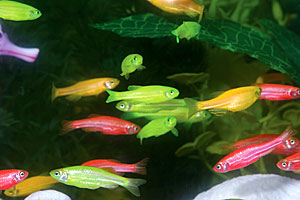
\includegraphics[width=\linewidth]{images/danio}
\caption{'Glofish':"Peces cebra"(\textit{Danio rerio}) que expresan proteínas fluorescentes GFP, YFP y RFP que actúan en asociación con el gen \textit{mylz2} \cite{gong2003development, fox2008fda}}
%\label{fig:danio}
\end{figure}    
    
    Otro caso importante de mascotas genéticamente modificadas es el de los gatos hipoalergénicos, actualmente en desarrollo por la empresa Felix Pets en EEUU. La expresión de la proteína Fel-dI (principal alérgeno, responsable del 90\% de los casos de alergia a gatos en humanos) se puede inhibir, silenciando el gen que la produce mediante la inserción de una secuencia llamada \textit{neo-r} en el primer o segundo intrón del gen\cite{avner2012method, butt2012hypoallergenic}. 
  
\section{Implicancias Bioéticas y Legales de la Transfección}

Como hemos visto, la transfección tiene múltiples aplicaciones con enorme potencial para mejorar la nutrición y la salud a nivel global. Sin embargo, estas ventajas no garantizan su aceptación pública.


%----------------------------------------------------------------------------------------
%	REFERENCE LIST
%----------------------------------------------------------------------------------------

\bibliographystyle{unsrt}
\bibliography{referencias}

%----------------------------------------------------------------------------------------

\end{document}
